\documentclass[tikz,border=10pt]{standalone}
\usepackage{tikz}
\usepackage{gensymb}
\usetikzlibrary{calc,angles,intersections}
\usepackage{tikz-dimline} % Import tikz-dimline package

\begin{document}
%Q1
    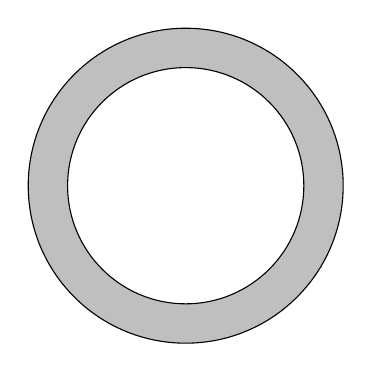
\begin{tikzpicture}
    
    % Outer circle
    \filldraw[fill=gray!50] (0,0) circle (2cm);
    
    % Inner circle
    \draw[fill=white] (0,0) circle (1.5cm);
    
    \end{tikzpicture}

%Q2
    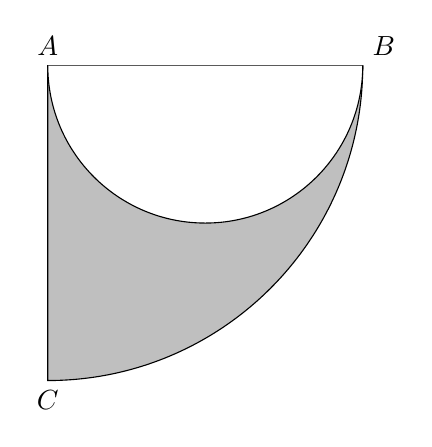
\begin{tikzpicture}
    \coordinate[label=above:$A$] (A) at (0,0);
    \coordinate[label=below:$C$] (C) at (0,-4);
    \coordinate[label=above right:$B$] (B) at (4,0);

    \draw (C)--(A)--(B);
    \draw[fill=gray!50] (B) arc[start angle=0, end angle=-90, radius=4] -- (C) -- (A) -- cycle;

    \draw[fill=white] (B) arc[start angle=0, end angle = -180, radius=2];
    \end{tikzpicture}

%Q3
    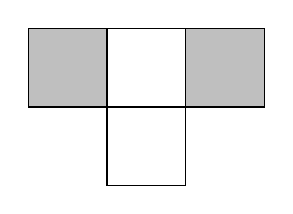
\begin{tikzpicture}

    % Top row of squares
    \draw[fill=gray!50] (0,0) rectangle (1,1);
    \draw (1,0) rectangle (2,1);
    \draw[fill=gray!50] (2,0) rectangle (3,1);
    
    % Middle square of the second row
    \draw (1,-1) rectangle (2,0);
    
    \end{tikzpicture}

%Q4
    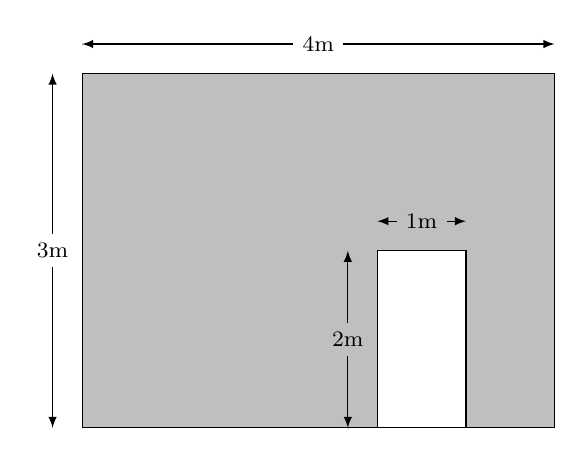
\begin{tikzpicture}[scale=1.5]

    % Draw rectangles
    \draw[fill=gray!50] (0,0) rectangle (4,3);
    \draw[fill=white] (2.5,0) rectangle (3.25,1.5);
    
    % Dimensions using tikz-dimline
    
    % Length dimension for the larger rectangle
    \dimline[label style={sloped=false}, line style={<->,>=latex, scale =2}, extension start length=0, extension end length=0]{(0,3.25)}{(4,3.25)}{\footnotesize 4m}


    % Height dimension for the larger rectangle
    \dimline[label style={sloped=false}, line style={<->,>=latex, scale =2}, extension start length=0, extension end length=0]{(-0.25,0)}{(-0.25,3)}{\footnotesize 3m}


    % Length dimension for the smaller rectangle
    \dimline[label style={sloped=false, fill=gray!50}, line style={<->,>=latex, scale =2}, extension start length=0, extension end length=0]{(2.5,1.75)}{(3.25,1.75)}{\footnotesize 1m}
    % Height dimension for the smaller rectangle
    \dimline[label style={sloped=false, fill=gray!50}, line style={<->,>=latex, scale =2}, extension start length=0, extension end length=0]{(2.25,0)}{(2.25,1.5)}{\footnotesize 2m}
\end{tikzpicture}

\end{document}
